\section{Komplexe Funktionen (Abbildungen)}

\vspace{-0.2cm}

$$ f: \: \mathbb{D}_f \subseteqq \mathbb{C}  \: \rightarrow \: \mathbb{W}_f \subseteqq  \mathbb{C}, \: z  \mapsto w = f(z) $$

\begin{itemize}[itemsep=0.2cm]
    \item Winkeltreue für komplex differenzierbare Funktion mit $f'(z) \neq 0$ \\
        \textrightarrow\ Drehstreckung mit Drehwinkel $\arg[f'(z)]$ und Streckfaktor $\vert f'(z) \vert$
    \item Die Ableitung $f'(z)$ beschreibt, was lokal im Punkt $z$ passiert \\
        \textrightarrow\ Streckfaktor und Drehwinkel im Punkt $z$ \\
        Beispiel: $f'(z) = \frac{1}{2}\jimg$ \quad \textrightarrow\ Steckung um $\frac{1}{2}$ und Drehwinkel $\frac{\pi}{2}$
\end{itemize}

   

\subsubsection{Parametergleichung von Bildkurven}

Parametergleichung einer Bildgeraden kann \textbf{immer} ermittelt werden!

\smallskip

\begin{tabular}{ll}
    waagerechte Gerade: & $z = z(r) = r + \jimg c_2$ \quad mit $r \in \mathbb{R}$ \\
    senkrechte Gerade:  & $z = z(r) = c_1 + \jimg s$ \quad mit $r \in \mathbb{R}$
\end{tabular}

\smallskip

\textrightarrow\ in $w = f(z) $ so einsetzen und ausrechnen / vereinfachen \\
\textrightarrow\ Beispiel-Resultat:  $w = (r^2 - c^2) + \jimg 2 r c$


\subsubsection{Koordinatengleichung von Bildkurven}

Kann nur bei \textbf{einfachen} Parametergleichungen ermittelt werden! \\
\textbf{Vorgehen:} In GlSys Parameter $r$ eliminieren 


\example{Koordinatengleichung von $\bm{w = (r^2 - c^2) + \jimg 2rc}$}

\begin{minipage}{0.35\linewidth}
    \begin{tabular}{| l |}
        $w_1 = r^2 - c^2$ \\
        $w_2 = 2rc$
    \end{tabular}
\end{minipage}
\hfill
\begin{minipage}{0.3\linewidth}
    $r = \frac{w_2}{2c}$ \\
    \textrightarrow\ einsetzen in $w_1$
\end{minipage}
\hfill
\begin{minipage}{0.25\linewidth}
    $w_1 = \frac{w_2^2}{(2c)^2} - c^2$
\end{minipage}

\columnbreak


\subsection{Lineare Funktion}

\vspace{-0.2cm}

$$ f: \: z \mapsto w = f(z) = az + b \quad \text{mit } a, \, b \in \mathbb{C} \text{ und } a \neq 0 $$

\begin{itemize}[itemsep=0.1cm]
    \item für $a = 1$ eine Translation um den Ortsvektor $\vec{b}$
    \item für $a \neq 1$ eine Drehstreckung mit Zentrum $\frac{b}{1-a}$, dem Drehwinkel $\arg(a)$ und dem Streckfaktor $\vert a \vert$
\end{itemize}

\vspace{-0.1cm}

\begin{center}
    \includegraphics[width=0.85\linewidth]{images/lineare_abbildung.png}
\end{center}

\vspace{-0.1cm}


\subsection{Quadratfunktion / Wurzelfunktion}

\begin{tabular}{ll}
    $\bm{f(z) = z^2}$       & Verdoppelung des Winkels $\arg(z)$ und Quadrierung des \\  \medskip
                            & Abstandes zum Ursprung $\vert z \vert ^2$ \\
    $\bm{f(z) = \sqrt{w}}$  & Halbierung des Winkels $\arg(z)$ und (relle) Wurzel des Abstandes \\
                            & zum Ursprung $\vert z \vert$
\end{tabular}

\medskip


\para{Quadratfunktion (kartesische Koordinaten)}

\begin{center}
     \includegraphics[width=0.85\linewidth]{images/quadratische_abbildung.PNG}
\end{center}
   
\vspace{-0.2cm}


\para{Quadratfunktion / Wurzelfunktion (Polarkoordinaten)}

\begin{center}
    \includegraphics[width=0.85\linewidth]{images/quadratische_abbildung_2.PNG}
\end{center}

\vspace{-0.2cm}


\subsubsection{Eigenschaften der Quadrat- und Wurzelfunktion}

\begin{itemize}
    \item rechte Hälfte der $z$-Ebene wird schon auf ganze $w$-Ebene abgebildet
    \item Doppelwertig, wenn linke Hälfte auch noch abgebildet wird
    \item bijektiv, bei 2-blättriger Riemann'scher Fläche
    \item Quadratfunktion überall winkeltreu ausser im Ursprung, weil dort $f'(z) = 2 z = 0$
    \item Wurzelfunktion überall winkeltreu ausser im Ursprung, weil $f'(z) = \frac{1}{2 \sqrt{z}}$ nicht definiert
\end{itemize}


\subsection{Potenzfunktion / Wurzelfunktion} 

\begin{tabular}{ll}
    \medskip
    $\bm{f(z) = z^n}$           & $n$-facher Winkel von $\arg(z)$ und Abstand $\vert z \vert ^n$ zum Ursprung \\ 
    $\bm{f(z) = \sqrt[n]{w}}$   & $n$-ter Teil des Winkels $\arg(z)$ und (relle) $n$-te Wurzel des \\
                                & Abstandes zum Ursprung $\vert z \vert$ \\
\end{tabular}

\begin{center}
    \includegraphics[width=0.8\columnwidth]{images/potenzfunktion.png}
\end{center}


\subsubsection{Eigenschaften der Potenz- und Wurzelfunktion}

\begin{itemize}
    \item bijektiv, bei $n$-blättriger Riemann'scher Fläche
    \item Beide Funktionen überall winkeltreu ausser im Ursprung
\end{itemize}


\subsection{Kreisspiegelung}

\vspace{-0.2cm}

$$ f: \: z \mapsto w = \frac{1}{\overline{z}} $$

\begin{tabular}{llllll}
    Abstand: & $\vert w \vert = \frac{1}{\vert z \vert }$ & &  Winkel: & $\arg(w) = \arg(z)$
\end{tabular}


\subsubsection{Eigenschaften der Kreisspiegelung}

\begin{itemize}
    \item bijektiv auf $\mathbb{C} \: \cap \: \lbrace \infty \rbrace$
    \item winkeltreu (bis auf das Vorzeichen)
    \item Geraden / Kreise gehen in Geraden / Kreise über
    \item Einheitskreis ist ein \textbf{Fixpunktkreis}
    \item Rand eines Kreises geht in den Rand des Bildkreises über
\end{itemize}
        

\subsubsection{Vorgehen Bildkurve / Bildfläche zeichnen}

\begin{minipage}[t]{0.55\linewidth}
    \includegraphics[width=\linewidth, align=t]{images/kreisspiegelung.png}
\end{minipage}
\hfill
\begin{minipage}[t]{0.43\linewidth}
    \raggedright

    \begin{enumerate}[itemsep=0.2cm]
        \item Ist  Bild eine Gerade oder ein Kreis?
        \item Gibt es Fixpunkte? (Einheitskreis)
        \item Abstand zu Ursprung auf Strahl reziprok
        \item Symmetrien beachten
        \item Fläche schraffieren: geeigneten Punkt aus Originalfläche abbilden
    \end{enumerate}

    \medskip

    \textbf{Hinweis:} Bei Bedarf Originalkurve in Kreise und Geraden zerlegen!
\end{minipage}

\columnbreak


\subsection{Kehrwertfunktion}

\vspace{-0.2cm}

$$ f: \: z \mapsto w = \frac{1}{z} $$

\begin{tabular}{lllllll}
    Abstand: & $\vert w \vert = \frac{1}{\vert z \vert }$ &  & & Winkel: & $\arg(w) = - \arg(z)$
\end{tabular}

\smallskip

\textbf{ \textrightarrow\ Grosse Ähnlichkeit zur Kreisspiegelung!}

% NOTE: Anregung / Idee für die Grafiken von Fabian Steiner
\begin{minipage}[c]{0.41\columnwidth}
    \begin{center}
    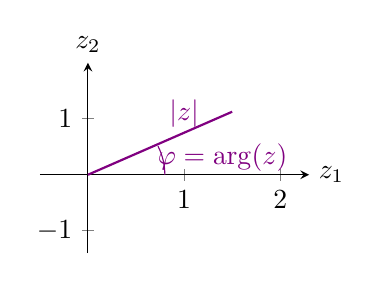
\begin{tikzpicture}
        [
            scale = 1.0,
            >=latex
        ]
        \begin{axis}[
            xmin=-0.5,
            xmax=2.3,
            ymin=-1.4,
            ymax=2,
            width=5cm,
            height=4cm,
            axis x line=middle, 
            axis y line=middle, 
            xtick={0, 1, 2},
            xticklabels={$0$, $1$, $2$},
            ytick={-1, 0, 1},
            x label style={anchor=west},
            xlabel={$z_1$}, 
            y label style={anchor=south},
            ylabel={$z_2$}
        ]
        
        \addplot[violet, thick, domain=0:1.5] {0.75*x};
        \draw[violet] (0.8, 0) arc[start angle=0, end angle=27, radius=0.8cm];
        \node[violet] at (1.4, 0.3) {$\varphi = \arg(z)$};
        
        \node[violet] at (1, 1.1) {$|z|$};

        \end{axis}
    \end{tikzpicture}
\end{center}
\end{minipage}
\hfill
\begin{minipage}[c]{0.08\columnwidth}
    $$ \underrightarrow{w = \frac{1}{z}} $$
\end{minipage}
\hfill
\begin{minipage}[c]{0.41\columnwidth}
    \begin{center}
    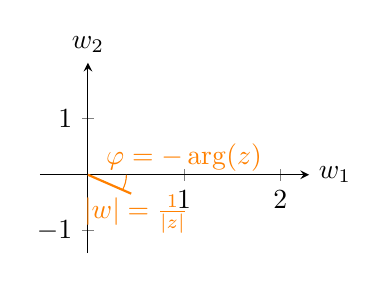
\begin{tikzpicture}
        [
            scale = 1.0,
            >=latex
        ]
        \begin{axis}[
            xmin=-0.5,
            xmax=2.3,
            ymin=-1.4,
            ymax=2,
            width=5cm,
            height=4cm,
            axis x line=middle, 
            axis y line=middle, 
            xtick={0, 1, 2},
            xticklabels={$0$, $1$, $2$},
            ytick={-1, 0, 1},
            x label style={anchor=west},
            xlabel={$w_1$}, 
            y label style={anchor=south},
            ylabel={$w_2$}
        ]
        
        \addplot[orange, thick, domain=0:0.45] {-0.75*x};
        \draw[orange] (0.4, 0) arc[start angle=0, end angle=-28, radius=0.4cm];
        \node[orange] at (1, 0.3) {$\varphi = -\arg(z)$};
        
        \node[orange] at (0.5, -0.7) {$|w| = \frac{1}{|z|}$};

        \end{axis}
    \end{tikzpicture}
\end{center}
\end{minipage}


\subsection{Exponentialfunktion / Logarithmusfunktion}

\vspace{-0.2cm}

$$ \e^z = \e^{z_1} \cdot \e^{\jimg z_2} = \e^{z_1} \cjs(z_2) \qquad \qquad  
\Ln(z) = \ln(\vert z \vert) + \jimg \arg(z) $$

\textrightarrow\ Der Nullpunkt (Ursprung) wird \textbf{nicht} abgebildet!

\begin{center}
    \includegraphics[width=0.85\linewidth]{images/exponentialfunktion.PNG}
\end{center}

\begin{itemize}
    \item Horizontale Geraden: Stahlen von Ursprung weg
    \item Vertikale Geraden: Kreise um Ursprung
\end{itemize}


\subsubsection{Eigenschaften der Exponential- und Logarithmusfunktion}

\begin{itemize}
    \item bijektiv, bei $\infty$-blättriger Riemann'scher Fläche ($2 \pi \jimg$-periodisch) ausser im Punkt $0$ (weil $\e^z \neq 0$)
    \item Exponentialfunktion $\e^z$ überall winkeltreu
    \item Umkehrfunktion $\Ln(w)$ überall in $\mathbb{D}_f$ winkeltreu ($\mathbb{C} \: \diagdown \; \lbrace 0 \rbrace$)
\end{itemize}


% Die Möbiustransformation ist Inhalt von Fabin Steiner 
% reformatting: Simone Stitz
\subsection{Möbisutransformation}

Die Möbiustransformation ist eine veralgemeinerung der Kehrwertsfunktion:
$$ f(z) = w = \frac{az + b}{cz + d} \qquad \qquad \text{Umkehrfunktion: } f(w) = z =\frac{-dw + b}{cw - a} $$
$a, \, b, \, c, \, d \in \mathbb{C}, \; c \neq0$ \& $ad - bc\neq 0$ \textrightarrow\ sonst wäre $f$ konstant


\smallskip

\resizebox{1\linewidth}{!}{%
\begin{circuitikz}
\tikzstyle{every node}=[font=\normalsize]
\draw [->, >=Stealth] (3.5,11.25) -- (6.5,11.25);
\node [font=\normalsize] at (4.75,11.5) {\textbf{$u=cz+d$}};
\node [font=\normalsize] at (5,11) {\textbf{lineare Funktion}};
\node [font=\normalsize] at (3,11.25) {\textbf{$f$: z}};
\draw [->, >=Stealth] (7.5,11.25) -- (10.5,11.25);
\node [font=\normalsize] at (8.75,11.5) {\textbf{$v=\frac{1}{u}$}};
\node [font=\normalsize] at (9,11) {\textbf{Kehrwertfunktion}};
\node [font=\normalsize] at (7,11.25) {\textbf{u}};
\draw [->, >=Stealth] (11.5,11.25) -- (14.5,11.25);
\node [font=\normalsize] at (12.75,11.5) {\textbf{$w=\frac{bc-ad}{c}v+\frac{a}{d}$}};
\node [font=\normalsize] at (13,11) {\textbf{lineare Funktion}};
\node [font=\normalsize] at (11,11.25) {\textbf{$v$}};
\node [font=\normalsize] at (14.75,11.25) {\textbf{w}};
\end{circuitikz}
}%


\subsubsection{Eigenschaften der Möbiustransformation}

\begin{itemize}
    \item Die Möbiustransformation ist winkel- und kreistreu
    \item Die Umkehrfunktion ist wieder eine Möbiustransformation \\
        \textbf{Achtung:} Es sind nur 3 Parameter! \textrightarrow\ ein Parameter kann gekürtzt werden
\end{itemize}

% Ende Code Fabian